\documentclass[a4paper,fleqn]{cas-dc}

% CAS loads STIX when available. Use Latin Modern only on its fallback path;
% replacing STIX symbol fonts after its mathcodes are set corrupts operators.
\IfFileExists{stix.sty}{}{\usepackage{lmodern}}
% Keep the source package self-contained: CAS's optional email icon is external.
\ExplSyntaxOn
\bool_gset_true:N \g_stm_nologo_bool
\ExplSyntaxOff

\usepackage[authoryear,round]{natbib}
\usepackage{booktabs}
\usepackage{tabularx}
\usepackage{array}
\usepackage{listings}
\usepackage{xcolor}
\usepackage{soul}
\usepackage{tikz}
\usetikzlibrary{arrows.meta}

% Coauthor review convention: yellow BAJ comments; orange MES corrections/additions.
\newcommand{\baj}[1]{{\sethlcolor{yellow}\hl{BAJ: #1}}}
\newcommand{\mes}[1]{{\sethlcolor{orange}\hl{MES: #1}}}
% Continue the same orange addition across normally typeset, breakable citations.
\newcommand{\mescont}[1]{{\sethlcolor{orange}\hl{#1}}}
\soulregister\citep7
\soulregister\citet7
\soulregister\ref7
\soulregister\texttt7
\soulregister\path7

\usepackage{amsmath,amssymb}
\usepackage{graphicx}
\usepackage{url}
\usepackage{microtype}
\usepackage{placeins}
\usepackage{enumitem}
\setlength{\emergencystretch}{1em}

\newcolumntype{Y}{>{\raggedright\arraybackslash}X}
\newcommand{\tool}{\textsc{LEAP}}
\newcommand{\bluebook}{\emph{Interactive Bluebook}}
\soulregister\bluebook0
\soulregister\tool0
\lstset{basicstyle=\ttfamily\scriptsize,showstringspaces=false,columns=fullflexible,keepspaces=true,breaklines=false,frame=single,numbers=none,captionpos=b,aboveskip=\intextsep,belowskip=\intextsep,xleftmargin=\fboxsep,xrightmargin=\fboxsep}
\hypersetup{colorlinks=true,linkcolor=blue,citecolor=blue,urlcolor=blue}

% Journal-specific preprint footer; Elsevier class files remain unmodified.
\ExplSyntaxOn
\cs_set:Npn \__first_footerline:
{
  \group_begin:
  \small
  \sffamily
  \ifnum\theblind>0\relax
  \else
    \__short_authors: :~
  \fi
  { \rmfamily \itshape Preprint~submitted~to~Journal~of~Systems~and~Software }
  \group_end:
}
\ExplSyntaxOff

\begin{document}
\let\WriteBookmarks\relax
\def\floatpagepagefraction{1}
\def\textpagefraction{.001}

\shorttitle{Explanation-Fidelity Audit in LEAP}
\shortauthors{M.O. Mouawad and B. Jones}

\title[mode=title]{Independent Evaluation of an Explanation-Fidelity Audit in LEAP: Construct Refinement and Checker Failure Modes}

\author[1]{Meshaal Obaid Mouawad}[auid=001,orcid=0000-0002-1152-8324]
\cormark[1]
\ead{mm4922@msstate.edu}

\author[1]{Bryan Jones}[auid=002,orcid=0000-0002-5807-8797]
\ead{bjones@ece.msstate.edu}

\affiliation[1]{organization={Department of Electrical and Computer Engineering, Mississippi State University},city={Mississippi State},postcode={39762},state={MS},country={USA}}
\cortext[cor1]{Corresponding author: Meshaal Obaid Mouawad}

\begin{abstract}[]
\baj{Given the brevity, avoid the bolded headings; instead, write a sentences which naturally lead from one topic to the next.}
\mes{the bold was deleted}
Source-linked documentation of enterprise key performance indicators (KPIs) can misdescribe the calculations used to produce business reports. We present an explanation-fidelity audit that compares LEAP's Interactive Bluebook with its implementation evidence and traces discrepancies to the generating mechanisms. Three independent reviewers assess four candidate dimensions across 28 KPI dossiers. Their judgments support two dimensions: source-role accuracy, which asks whether an explanation correctly identifies what a source element does, and condition disclosure, which asks whether it communicates conditions that change calculation behavior. Agreement is $\kappa=0.407$ and $\kappa=0.553$, respectively. The automated source-role checker detects 2 of 16 reviewer-majority failures (12.5\% recall). Across 10 eligible condition cases, precision is 40\% under a source-visibility criterion and 100\% under a reader-facing criterion, with 100\% recall under both. Comparison of the Yield and Gross Margin dossiers shows that source-linkage verification passes while semantic inspection identifies incorrect source-role descriptions and incomplete safeguards. Generator tracing locates the publication mechanisms responsible for these discrepancies. The audit provides an inspectable basis for connecting business-facing KPI explanations to executable evidence and identifying where automated documentation checks require improvement.
\end{abstract}

\begin{keywords}
software documentation \sep program comprehension \sep provenance \sep traceability \sep key performance indicators \sep explanation fidelity \sep knowledge engineering
\end{keywords}
\maketitle
\hypersetup{pdfauthor={Meshaal Obaid Mouawad; Bryan Jones}}

\section{Introduction}

\baj{This paper needs a proper introduction: begin by stating the problem, then why this approach solves the problem. The material here comes after these paragraphs. Define KPIs, why these are important, how they're not traditionally linked to code, etc.}

\baj{[Tying to the need for LEAP...] Therefore,}

Enterprise performance reporting relies on agreement between the metric described in a business Bluebook and the calculation executed by software. Business teams use the description to interpret results and choose actions; technical teams implement the inputs, formulas, and conditions that produce them. A discrepancy creates both a software-verification problem and a barrier to shared understanding. This paper addresses that problem through an explanation-fidelity audit of LEAP documentation. Evidence from 28 dossiers and three independent reviewers supports two dimensions: source-role accuracy asks whether an explanation correctly identifies what a source element does; condition disclosure asks whether it communicates conditions that change calculation behavior. Together, they examine whether business-facing explanations preserve implementation meaning.

\mes{Key performance indicators (KPIs) are quantifiable measures used to evaluate progress toward strategic and operational objectives. Their meaning connects a business definition of what should be measured with the calculation that produces the reported value. In software-based reporting, this connection includes the inputs, formula, and conditions implemented in source code. Understanding a KPI therefore requires access to both its business interpretation and the computational decisions that determine its value} \citep{Mate2017,RoldanGarcia2021}.

\mes{The manual workflow motivating LEAP separates these representations across people and artifacts. A business analyst specifies the indicator, a developer translates that specification into executable logic, and a separate documentation effort records the calculation in a Bluebook for business readers. When a value is questioned or an implementation changes, the team must trace between the documented definition and the code to determine which inputs, formula, and exceptional cases apply. The code produces the number; the Bluebook communicates its meaning. Documentation maintenance and code--comment consistency research establish the need to maintain this relationship as software evolves} \citep{Aghajani2019,Wen2019,Xu2024}.

The difference between the two representations can change the meaning of the reported metric. In the Gross Margin case examined here, the declared business formula and the executable expression differ by at least 100 percentage points throughout the strictly positive input domain. In the Yield case, the implementation returns zero for non-positive feedstock, a condition omitted from the published safeguards. These examples show why business readers need an explanation of the implemented calculation alongside access to its source. The practical research problem is to make discrepancies between those representations visible and attributable to specific publication mechanisms.

\mes{LEAP (Literate Programming for Automated KPI Extraction) addresses this documentation problem by publishing a source-linked record for each KPI in an Interactive Bluebook. Its pipeline discovers KPI candidates, prepares formula and business-context fields, attaches provenance and review information, and presents these elements together with source explanations and safeguards. This shared record makes the relationship between a business definition and its implementation available for inspection. Its explanatory value depends on whether the published fields accurately communicate the roles and conditions of the retained evidence.}

This paper presents and independently evaluates an explanation-fidelity audit for the business--code connection published by LEAP. The audit compares source evidence with generated descriptions of its roles, conditions, conflicts, and review state. In this study, \emph{explanation fidelity} denotes the two publication dimensions supported by independent review: semantic source-role accuracy and communication of behavior-qualifying conditions. Root-cause analysis connects observed discrepancies to the generator mechanisms that produced them, making the evidence useful for interpreting the published KPI and identifying where its documentation requires repair.

Prior work establishes the underlying problems. Code--text consistency research measures divergence between source and documentation \citep{Wen2019,Xu2024,Eghbali2026}, and API-documentation research detects missing or inconsistent parameter, constraint, and exception directives \citep{Zhou2017}. \baj{What about traditional literate programming approaches, or documentation generators such as Doxygen, Javadoc, Rustdoc, etc.? These do an excellent job of code–text consistency.}

\mes{Literate programming provides an established foundation for connecting implementation with human-readable explanation. Knuth's WEB approach interleaves procedural code and narrative so that readers can follow a program's rationale and structure alongside its executable components} \citep{Knuth1984}.

\mes{Documentation generators provide further mechanisms for publishing source-connected explanations. Doxygen incorporates structured documentation comments, Javadoc associates documentation with Java declarations, and rustdoc compiles and runs suitable code examples as documentation tests} \citep{DoxygenManual,JavadocGuide,RustdocBook}.

\mes{LEAP applies this principle to the KPI as a shared knowledge record, assembling its business formula, executable evidence, explanatory fields, safeguards, and review state. This organization makes the relationship between business meaning and implementation inspectable. The present evaluation examines whether the generated fields preserve that relationship accurately.}

The contribution is a method for examining what happens when implementation evidence becomes business-facing documentation. It combines source-to-publication comparison, generator tracing, and independent reviewer judgments. This design distinguishes three questions: whether evidence remains accessible, whether its published interpretation preserves its meaning, and whether an automated rule detects the discrepancies identified by reviewers.

The evaluation supports source-role accuracy and condition disclosure as reproducible publication dimensions. It also identifies concrete differences between the requirements reviewers recognize and the rules used to check them: source-role recall is 12.5\%, and condition precision changes from 40\% to 100\% under the two observed disclosure criteria. The disagreement and authority results determine which additional checks are retained as LEAP-specific verification and which operationalization is rejected. These findings provide an empirical basis for choosing publication checks and directing improvements to their implementation.

These findings yield three contributions:
\begin{enumerate}[leftmargin=*]
\item a source-to-publication audit that connects business-facing KPI formulas and explanations to executable evidence and traces discrepancies to generator mechanisms;
\item an independent assessment of four candidate dimensions on 28 dossiers, retaining source-role accuracy and condition disclosure, narrowing disagreement to explicit-conflict routing, and rejecting review-authority consistency; and
\item reproducible comparisons of source-linkage verification, field-level publication findings, and reviewer judgments that expose rule-coverage failures and condition-definition sensitivity.
\end{enumerate}
\section{Related Work and Candidate Check Derivation}
\subsection{Behavioral fidelity and source roles}
Software documentation remains difficult to create and maintain \citep{Aghajani2019}. Traceability identifies relationships between documentation and software artifacts \citep{MaderGotel2012}; code-comment inconsistency studies show that linked text can still diverge from code semantics \citep{Wen2019,Xu2024}. Eghbali et al. formalize code-documentation equivalence around accurate and complete description of program behavior \citep{Eghbali2026}. Zhou et al. compare API code with parameter-constraint and exception directives to detect documentation defects \citep{Zhou2017}. \baj{Need another sentence– “This research demonstrates the ongoing problem of failed code–documentation equivalence. The LEAP system addresses this problems by...”}
\mes{These studies establish that documentation can remain linked to code while describing its behavior incompletely or incorrectly. LEAP makes this relationship inspectable by presenting KPI source evidence alongside generated formula, explanation, and safeguard fields. The present audit evaluates whether those fields preserve the meaning of the evidence they describe.}
These results motivate source-role accuracy and condition disclosure as publication obligations.

LEAP brings these consistency requirements into the publication of a business metric. \baj{Then why reference these as related works?}
\mes{These works provide the semantic requirements applied here: an explanation should identify source elements accurately and communicate conditions that qualify program behavior. The LEAP case study evaluates those requirements in generated KPI documentation.} Each audited dossier already contains a source link; the question is whether generated publication fields preserve the role and qualifying conditions of that linked evidence. This fixed-provenance design separates link correctness from publication semantics and permits independent evaluation of the publication transformation itself.

\subsection{Disagreement, evidence roles, and authority}
Nuseibeh et al. show that inconsistency can be retained and managed rather than silently eliminated \citep{Nuseibeh2001}. SEPIO \baj{A bit confusing – SEPIO is a new acronym not defined yet, but appears in the referenced paper. State more explicitly that SEPIO is the name of the system in this paper. The same goes for the following acronyms.} \mes{(Scientific Evidence and Provenance Information Ontology), the evidence model introduced by Brush et al.,} represents claims, evidence lines, data, methods, tools, agents, and supporting or refuting relations \citep{Brush2016}; ECO \mes{(Evidence and Conclusion Ontology)} distinguishes evidence and assertion-method types \citep{Giglio2019}. These precedents motivate explicit preservation of representation disagreement and separation between evidence state and the authority communicated by surrounding prose. \baj{Tie this back to LEAP. How does LEAP do this? Does it merely follow this existing work, or does it provide a new contribution?}
\mes{LEAP applies these principles by retaining source representations, explicit conflict signals, and review states within the same dossier. The evaluation distinguishes this implementation from the broader concepts that motivate it: preserving an explicitly marked conflict supports a routing verification, while independent reviewer agreement determines whether disagreement and review-authority judgments support reproducible publication dimensions.}

PROV \mes{(the World Wide Web Consortium's family of provenance specifications)} supplies interoperable entity--activity--agent provenance and formal validity constraints \citep{Missier2013,W3CProvConstraints2013}. OneProvenance reconstructs dynamic query lineage from database events \citep{Psallidas2023}. ESDPKI \mes{(Enterprise Spatial Data Provenance Knowledge Infrastructure)} adds semantic provenance, validation-gated ingestion, publication, governance, and access controls in an enterprise infrastructure \citep{Sadiq2026}. Together, these systems establish provenance, validation, and governance as distinct information structures whose reader-facing communication can be audited. \baj{Again, how does this affect LEAP? How do you distinguish your contribution from earlier work? Same for following paragraphs.}
\mes{For LEAP, these distinctions identify information that the published dossier must communicate: where evidence originated, how it was transformed, and what review state accompanies it. The contribution evaluated here concerns the accuracy of that communication. Source links remain available while the audit examines whether the generated explanation preserves the source role, qualifying conditions, conflict signals, and review state.}

\subsection{Source-bound software knowledge}
ECK \mes{(Executable Code Knowledge)} defines source-bound executable knowledge with evidence, provenance, validation state, freshness, downstream projections, and projection-fidelity evaluation \citep{Gao2026}. Reversa preserves traceability, confidence, and explicit validation gaps in reconstructed specifications \citep{MacedoCosta2026}. The candidate checklist focuses on the publication transformation itself: source-role description, behavior-qualifying conditions, explicit representation conflict, and review/status language are each evaluated as potentially distinct publication checks.

\begin{table*}[t]
\centering
\caption{Literature basis and initial operationalization of the four candidate explanation-fidelity dimensions evaluated in this study.}
\label{tab:contract}
\begin{tabularx}{\textwidth}{@{}lYY@{}}
\toprule
Candidate dimension & Established basis & Initial LEAP operationalization \\
\midrule
Source-role accuracy & Code--text consistency and documentation equivalence \citep{Wen2019,Xu2024,Eghbali2026} & Flag a published explanation that assigns a source element the wrong syntactic/semantic role. \\
Condition disclosure & Completeness of behavioral/API directives \citep{Eghbali2026,Zhou2017} & For explicit zero/non-positive denominator guards, preserve the guarded variable and condition semantics. \\
Representation disagreement & Inconsistency management and conflicting evidence \citep{Nuseibeh2001,Brush2016} & For source evidence carrying an explicit conflict marker, preserve the conflict in review routing. \\
Review-authority consistency & Evidence/assertion roles, provenance validity, and validation-governance separation \citep{Giglio2019,W3CProvConstraints2013,Sadiq2026} & On unresolved dossiers, flag bounded certification-oriented wording. \\
\bottomrule
\end{tabularx}
\end{table*}

\baj{Summarize: while previous research shows the need for... LEAP therefore provides these needed enhancements, by... as detailed in the following section.}
\mes{Together, these studies motivate documentation that connects explanations to implementation evidence and preserves the meaning of that evidence during publication. LEAP provides a KPI dossier in which formulas, source context, safeguards, and review information can be inspected together. The following evaluation tests which proposed fidelity dimensions receive independent reviewer support and where the implemented checks fail.}

KPI semantics provide the domain context. Semantic KPI work formalizes indicator definitions and derivations \citep{Mate2017,RoldanGarcia2021,Diamantini2025}, and AFFECTK \mes{(the KPI-evolution framework introduced by Dominguez et al.)} makes traceability and consistency explicit during KPI evolution \citep{Dominguez2025}. The four initial candidates are evaluated where KPI representations meet executable source and publication state; the independent evidence determines which constructs survive and which automation requires redesign.
\baj{You need to show how LEAP improves on earlier designs, or offers new abilities. RQs about software behavior are less relevant here. What’s the core contribution LEAP provides in this context?}
\mes{The core contribution in this context is an empirical assessment of the transformation from executable KPI evidence to published business explanation. LEAP supplies the shared dossier on which that transformation can be inspected. The study separates the evidence supporting a proposed fidelity dimension from the performance of the checker implementing it, thereby identifying both reproducible publication obligations and concrete limitations of their automation.}
\section{Research Questions and Method}
The study asks:
\begin{description}[leftmargin=1.2cm,style=nextline]
\item[RQ1] Which \mes{discrepancies between source evidence and published KPI explanations} are exposed in the full 28-dossier LEAP output, and which generator mechanisms explain the repeated manifestations?
\item[RQ2] Which \mes{discrepancies in published KPI knowledge} persist or vary across an earlier project state and alternative input configurations?
\item[RQ3] Which candidate explanation-fidelity dimensions achieve reproducible independent reviewer agreement?
\item[RQ4] What checker failure modes and criterion sensitivities appear when the released rules are compared with independently produced reviewer labels?
\end{description}

\subsection{Claims and falsification conditions}
Table~\ref{tab:falsification} binds the study's major claims to observable evidence and an explicit overturning condition.

\begin{table*}[t]
\centering
\caption{Major claims, supporting evidence, and falsification conditions.}
\label{tab:falsification}
\begin{tabularx}{\textwidth}{@{}p{0.27\textwidth}YY@{}}
\toprule
Claim & Supporting evidence & Falsification condition \\
\midrule
Within the LEAP case study, source linkage can coexist with publication discrepancies. & Source-linked Yield and Gross Margin dossiers retain inspectable source evidence while direct comparison identifies role and condition discrepancies. & The claim fails if the retained evidence link is absent or direct source comparison removes the reported discrepancy. \\
Three root-caused LEAP generator mechanisms explain repeated primary-output manifestations. & Root-cause tracing maps lineage, safeguard, and certification-string manifestations to three shared generator mechanisms. & The claim fails if rerunning the released audit changes the manifestations or if repeated manifestations map to different generator mechanisms. \\
Independent review differentiates the candidate dimensions. & Three reviewers provide 112 guided cells; Fleiss' $\kappa$ ranges from 0.553 to \baj{Why does this render as *0.285?} $-0.285$ \mes{the minus sign was corrected}, and explicit-label sensitivity changes the disagreement result. & The claim fails if the preserved reviewer forms and deterministic aggregation reproduce uniform agreement across the four candidates. \\
The released source-role rule fails coverage, while condition-rule performance is criterion-sensitive. & Source-role recall is 12.5\% against reviewer majority. On the 10 checker-eligible condition cases, precision is 40\% under the source-visibility criterion and 100\% under the reader-facing criterion; recall is 100\% under both. & The claim fails if deterministic recomputation removes the source-role confusion matrix or the dual-criterion condition results. \\
\bottomrule
\end{tabularx}
\end{table*}

\subsection{Case-study system and publication pipeline}
LEAP is a source-to-publication system for KPI knowledge. Its \baj{[seems extraneous; do you means that this is frozen for publication purposes?] frozen research artifact} \mes{implementation} discovers KPI candidates from source files, prepares formula and business-context fields, attaches provenance and review information, and renders each selected KPI as an HTML dossier in the Interactive Bluebook. The dossier combines source context, formal formula presentation, developer-lineage prose, safeguards, ownership metadata, conflict signals, and a review state. This paper treats that rendered publication surface as the audit object and traces repeated publication findings back to the \baj{[Again, distracting from the goal of the sentence] frozen generator} generator implementation. \mes{the repeated frozen qualifier was deleted}

\begin{figure*}[t]
\centering
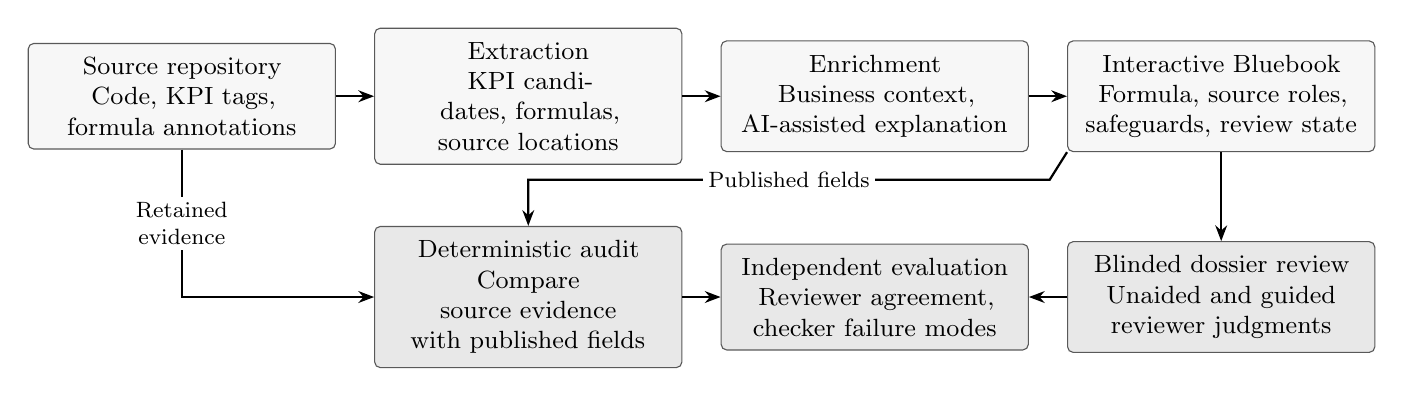
\begin{tikzpicture}[
  box/.style={draw=black!65,rounded corners=2pt,fill=black!3,align=center,text width=3.55cm,minimum height=1.15cm,inner sep=5pt,font=\small},
  study/.style={box,fill=black!9},
  flow/.style={-{Stealth[length=2mm]},thick},
  tag/.style={font=\footnotesize,fill=white,inner sep=2pt,align=center}]
\node[box] (source) at (0,0) {Source repository\\Code, KPI tags,\\formula annotations};
\node[box] (extract) at (4.4,0) {Extraction\\KPI candidates, formulas,\\source locations};
\node[box] (enrich) at (8.8,0) {Enrichment\\Business context,\\AI-assisted explanation};
\node[box] (book) at (13.2,0) {Interactive Bluebook\\Formula, source roles,\\safeguards, review state};
\draw[flow] (source) -- (extract);
\draw[flow] (extract) -- (enrich);
\draw[flow] (enrich) -- (book);
\node[study] (audit) at (4.4,-2.55) {Deterministic audit\\Compare source evidence\\with published fields};
\node[study] (compare) at (8.8,-2.55) {Independent evaluation\\Reviewer agreement,\\checker failure modes};
\node[study] (review) at (13.2,-2.55) {Blinded dossier review\\Unaided and guided\\reviewer judgments};
\draw[flow] (source.south) |- node[tag,pos=.25]{Retained\\evidence} (audit.west);
\draw[flow] (book.south) -- (review.north);
\draw[flow] (book.south west) -- ++(-.22,-.35) -| node[tag,pos=.25]{Published fields} (audit.north);
\draw[flow] (audit) -- (compare);
\draw[flow] (review) -- (compare);
\end{tikzpicture}
% Workflow adapted from the approved proposal, chapter4.tex and Figuers/image11.svg.
\caption{\protect\mes{LEAP's source-to-publication workflow (upper row) and the dossier audit and independent reviewer comparison performed in this study (lower row). Source evidence and published explanations meet in the audit, making the business--implementation connection inspectable.}}
\label{fig:leap-pipeline}
\end{figure*}

\subsection{Case-study artifacts and within-system design}
\label{sec:artifacts}
\mes{Here, frozen denotes the fixed evaluation snapshot of the generator, inputs, and published pages used to reproduce the reported comparisons.}
The primary case-study artifact contains all 28 rendered dossier HTML pages produced by the frozen LEAP sample-project build. A public artifact copy at commit \texttt{5e697b5b} (full identity in the supplement) matches all 28 submitted pages byte-for-byte by SHA-256. The build contains 9 \emph{Validated} and 19 \emph{Needs Review} dossiers. These recorded states support the concrete LEAP certification-string analysis and also provide evidence for evaluating the broader review-authority candidate independently.

A separately archived earlier LEAP project state contains 18 rendered dossier HTML pages, including 6 \emph{Validated} and 12 \emph{Needs Review} dossiers. We use this archived state to test temporal persistence of named manifestations. Two further frozen LEAP input configurations use the same generator: a 38-file scenario-fixture scope producing 29 dossier publication sources and an 8-file challenge scope producing 8. These runs test input sensitivity. The unit of analysis is a generated dossier, and the audit operates on published source roles, formula-related conditions, conflict signals, and review-state language.

\paragraph{External adapter check.} Four official FastAPI tutorial sources and their generated OpenAPI 3.1 descriptions at fixed upstream identities \citep{FastAPI2026,OpenAPI31} verify that the source-role and declarative-condition adapters execute outside LEAP. This check is implementation evidence for adapter feasibility and is excluded from the independent construct evaluation.

\subsection{Deterministic operational rules}
\baj{Why are these rules sufficient? What inputs cause them to produce incorrect results?}
The released checker implements the following four initial rules; the independent evaluation determines their empirical status.
\mes{The four rules are bounded operationalizations of the literature-derived candidates in Table~\ref{tab:contract}. They are evaluated as hypotheses about detectable publication failures. Author-specified controls test whether each rule implements its stated criterion, while independent dossier judgments test how much of the observed failure set it captures. The latter comparison exposes a substantial coverage limitation: the source-role rule detects only 2 of 16 reviewer-majority failures.}
\begin{enumerate}[leftmargin=*]
\item \textbf{Source-role accuracy.} A failure is recorded when a comment or docstring is assigned an executable role, or when a SQL \texttt{CAST} type is labeled as the output alias instead of the actual alias. The rule scans published developer-lineage pairs.
\item \textbf{Executable-guard disclosure.} Eligibility covers explicit zero or non-positive denominator \baj{Why is a negative denominator a problem? For zero checks, does it also include values that are close to zero? What about other places where the answer is problematic, such as negative values for a square root, negative values for an inverse log, invalid values for arc sin/cos/tan, etc.?} guards expressed as \texttt{NULLIF(variable,0)} or an \texttt{if}-family comparison to zero. Preservation requires reader-facing safeguard text to communicate zero/non-positive handling and bind the guarded variable to the denominator displayed in the formal formula. A \texttt{<= 0} guard requires non-positive semantics; zero-only wording fails the rule.
\mes{A negative nonzero denominator is mathematically valid. The obligation here arises from the implemented branch: the Yield source returns zero when feedstock input is non-positive. Consequently, zero-only safeguard wording omits part of the implemented condition.}
\item \textbf{Representation-disagreement candidate.} The released rule covers pages whose retained source explicitly carries a conflict, mismatch, or inversion marker and checks preservation through \emph{Needs Review} plus a Review Queue. The independent evaluation tests whether this narrow rule supports a broader disagreement construct.
\item \textbf{Review-authority candidate.} The released rule checks unresolved \emph{Needs Review} dossiers for bounded certification-oriented wording such as ``Certified metric dossier'', ``certified calculation expression'', or ``Print Certified Dossier''. Independent reviewer reliability determines this candidate's empirical disposition.
\end{enumerate}
The complete guard table and all line-level role findings are emitted by the scripts for inspection, and Table~\ref{tab:contract} records the literature basis of each initial candidate.

\subsection{Evaluated checker and conformance tests}
The reported evaluation uses the R3 \baj{does this mean rule 3?} \mes{(the third protocol revision)} audit protocol and the R4 \mes{(the fourth implementation revision)} checker. The evaluated implementation compares published roles and names with their source counterparts, requires a nonempty displayed denominator, and tests safeguard wording for variable correspondence, handling semantics, and contradictions. The conformance tests below exercise these requirements through prespecified control outcomes.

The released checker is exercised in two conformance-test layers against author-specified control-oracle tables stored separately from checker output. Eighteen rule fixtures exercise correct and substituted source roles, correct/missing/wrong denominator binding, contradictory or disabled safeguard prose, zero-only loss of non-positive semantics, preserved/suppressed conflict routing, certification beside unresolved status, benign controls, and N/A behavior. Fourteen artifact-derived controls add five unchanged baselines, eight substitutions of extracted inputs, and one document-level HTML mutation reparsed through the same publication adapter used for the archived LEAP page. All 32 oracle-labeled outcomes match; the 30 binary Pass/Fail controls produce zero observed misses on deliberately introduced defects and zero observed false alarms on benign controls.
\baj{Reviews will be suspicious here – the test found no failures for any of the rules? This would be more convincing if failures are in areas that humans will catch, etc.}
\mes{Matching the control oracle includes returning Fail when a control is deliberately defective. Across the 32 controls, the expected outcomes comprise 19 Fail, 11 Pass, and two N/A labels. These results establish conformance to the specified control cases. Independent comparison on the original dossiers reveals the coverage limitation: the source-role checker misses 14 of the 16 reviewer-majority failures.}


\subsection{Independent reviewer evaluation and unaided baseline}
Three independent reviewers evaluated the same 28 dossier cases using blinded identifiers C01--C28. Reviewer packets excluded checker outputs, manuscript result tables, the organizer mapping key, and other reviewer responses. Phase A recorded unaided issue discovery. Phase B applied the four candidate dimensions and recorded Pass, Fail, or NA with evidence.

The returned Phase-A forms are complete for all 28 cases. In Phase B, reviewers left 94 of 336 possible obligation labels blank (28.0\%). All blanks occur in the applicability-dependent condition and disagreement columns: 40/84 condition labels and 54/84 disagreement labels. The primary analysis preserves the raw forms and maps these blanks to NA according to the collection protocol; every explicit Pass/Fail label remains unchanged. A sensitivity analysis is also reported for cells with three explicit labels.

For each case-dimension cell, a reviewer-majority label requires at least two matching labels; one three-way split remains unresolved. We report average pair agreement and Fleiss' $\kappa$ \citep{Fleiss1971}. We use reviewer majority as an independent comparison reference. Checker comparison is unconditional across the 28 cases: exact three-state agreement uses Pass/Fail/NA, and a binary defect confusion matrix treats reviewer-majority Fail as positive and Pass/NA as non-fail. This design exposes both checker underflagging and overflagging without conditioning performance on checker-defined eligibility sets.

Phase B followed Phase A on the same cases. The five cases that enter the majority issue set only in Phase B are inspected case-by-case to identify the source of the phase shift.

\subsection{Verification and root-cause procedure}
The primary audit verifies corpus size, SHA-256 identity, status counts, lineage pairs, guard instances, conflict routing, and certification wording. Primary, historical, robustness, and external scripts import the same released rule library for denominator binding, safeguard semantics, conflict routing, authority consistency, and source-role comparison where applicable. The primary guard inventory contains ten eligible guards and is produced directly by the scanner. The release verifier requires the control-oracle comparison and both checker-conformance execution layers to pass before accepting corpus summaries.

After classifying page manifestations, we inspect frozen generator source to determine whether repeated manifestations share one implementation cause. Root-cause evidence is accepted when one source mechanism explains the repeated page behavior. The supplement retains the exact generator excerpts and source hashes used for this trace.
\section{Results}
\subsection{LEAP case-study findings: three root-caused generator defects and preserved conflict routing}
The full 28-dossier case-study audit localizes three root-caused LEAP generator defects: lineage typing, guard-to-safeguard binding, and unconditional certification wording. It also verifies preserved conflict routing in all six eligible explicit-conflict dossiers. Table~\ref{tab:results} separates generator mechanisms from their page-level manifestations.

\begin{table*}[t]
\centering
\caption{Within-LEAP temporal persistence of generator manifestations and conflict routing.}
\label{tab:results}
\begin{tabularx}{\textwidth}{@{}lYY Y@{}}
\toprule
Class / mechanism & Current 28-dossier build & Earlier 18-dossier build & Interpretation \\
\midrule
Lineage typing defect & 4 dossiers; 12 manifestations & Same 4 dossiers; same 12 manifestations & Same classifier defect persists across the two archived project states \\
Guard-to-safeguard binding defect & 5 failures / 10 eligible guards & 4 failures / 9 eligible guards & Same generator weakness with one changed eligible outcome \\
Certification-wording template defect & 19 / 19 unresolved dossiers & 12 / 12 unresolved dossiers & Same unconditional template behavior appears on every unresolved page in each build \\
Conflict routing mechanism & Same 6 explicit-conflict dossiers, 6 / 6 preserved & Same 6 dossiers, 6 / 6 preserved & Intended routing behavior persists across all shared conflict cases \\
\bottomrule
\end{tabularx}
\end{table*}

The two alternative LEAP configurations show lineage and certification-wording findings while both eligible zero guards pass. The 29-dossier scenario build contains one lineage finding and certification-wording findings on all 11 unresolved dossiers; its one eligible zero guard passes. The 8-dossier challenge build contains one lineage finding and certification-wording findings on all six unresolved dossiers; its one eligible zero guard also passes. Generated conflict flags retain their review routing in both configurations. The guard result therefore varies with input configuration, whereas lineage and certification-wording findings recur.

\subsection{Root-cause localization}
The repeated LEAP manifestations map to three generator mechanisms. First, the developer-lineage classifier tests calculation/formula keywords before comment typing, leaves the ABAP \texttt{*} comment prefix outside its recognized comment prefixes, and applies a generic SQL \texttt{AS} pattern that can select a \texttt{CAST} type instead of the final alias. This classifier explains the source-role manifestations. The On-Spec Rate page provides a concrete SQL example: \texttt{CAST(... AS FLOAT) AS on\_spec\_percentage} is published as ``Output alias: maps this expression to FLOAT'', even though \texttt{on\_spec\_percentage} is the actual SQL alias and \texttt{FLOAT} is the cast type.

Second, safeguard generation recognizes \texttt{NULLIF} and selected equality-to-zero patterns and emits generic ``zero denominator'' language. Its output drops variable-to-denominator binding and \texttt{<= 0} semantics in the affected cases. This mechanism explains the five current guard failures while correctly aligned \texttt{NULLIF} cases pass.

Third, certification-oriented strings are emitted independently of review state in generator prose and the page template. That mechanism explains the 19/19 certification-wording findings on unresolved pages. Explicit conflict signals follow a separate routing path to \emph{Needs Review} and the Review Queue, producing the 6/6 preserved-conflict result.

\subsection{Checker conformance-test results}
The evaluated rule implementation matches all 18 predeclared rule fixtures and all 14 artifact-derived controls using the author-specified control labels. Changing the external query parameter from \texttt{query/item-query} to a header or wrong name triggers a source-role failure. Removing the displayed denominator, replacing safeguard prose with ``No zero handling is provided.'', stating that the zero guard is disabled, or reparsing a page whose explanatory sentence is replaced by a second ``Zero-Division Guard:'' heading triggers the guard rule. Suppressing a Review Queue entry from an explicit conflict and placing certification wording beside unresolved status are also detected. Across the 30 binary controls, the checker produces zero observed misses on defect controls and zero observed false alarms on benign controls; two additional fixtures produce their author-specified N/A outcomes.


\subsection{Independent reviewer evaluation and empirical refinement}
Across all 112 guided cells, average pair agreement is 0.634 and Fleiss' $\kappa$ is 0.446, with one unresolved cell. Per-candidate agreement is 0.553 for condition disclosure, 0.407 for source-role accuracy, 0.452 for disagreement preservation in the normalized analysis, and $-0.285$ for review-authority consistency. The authority result uses all 84 possible labels: reviewers left zero authority cells blank, so its $\kappa=-0.285$ is unconditional with respect to the blank-to-NA normalization procedure. The authority operationalization therefore fails inter-reviewer reliability \citep{Fleiss1971}.

Normalization materially affects the disagreement candidate. The 94 blank-to-NA mappings represent 28.0\% of the 336 possible reviewer labels, including 40/84 condition labels and 54/84 disagreement labels. On the seven disagreement cells with three explicit reviewer labels, $\kappa=-0.167$. The broad disagreement candidate is therefore removed from the retained explanation-fidelity construct. LEAP's narrower explicit-conflict-routing verification is reported separately as a system-specific routing check.

Table~\ref{tab:independent} reports unconditional checker comparison against reviewer-majority labels. The released source-role rule has a coverage failure: reviewer majority marks 16 failures while the checker flags four, producing TP=2, FP=2, FN=14, TN=10, precision 50\%, and recall 12.5\%. The condition rule yields TP=2, FP=3, FN=0, TN=22, precision 40\%, and recall 100\% against majority. Evidence inspection shows that all three apparent condition false positives are the same 2--1 criterion split, so Table~\ref{tab:condition_criteria} reports the condition rule under both observed disclosure criteria.

\begin{table*}[t]
\centering
\caption{Independent reviewer agreement and unconditional checker comparison. FAIL is the positive class. Precision and recall are computed against reviewer-majority labels on the fixed dossier set.}
\label{tab:independent}
\begin{tabularx}{\textwidth}{@{}lrrrrrrrrY@{}}
\toprule
Candidate & Fleiss' $\kappa$ & TP & FP & FN & TN & Precision & Recall & Exact / $n$ & Empirical disposition \\
\midrule
Source-role accuracy & 0.407 & 2 & 2 & 14 & 10 & 0.50 & 0.125 & 12/28 & Dimension retained; released rule fails coverage at 12.5\% recall. \\
Condition disclosure & 0.553 & 2 & 3 & 0 & 22 & 0.40 & 1.00 & 22/27 & Dimension retained; majority comparison reflects the source-visibility criterion in three disputed cells. \\
Disagreement candidate & 0.452 & 0 & 0 & 4 & 24 & -- & 0.00 & 24/28 & Broad construct removed; explicit-only sensitivity gives $\kappa=-0.167$; LEAP routing verification reported separately. \\
Review-authority candidate & $-0.285$ & 19 & 0 & 3 & 6 & 1.00 & 0.864 & 19/28 & Operationalization rejected; all 84 reviewer labels are explicit, so the negative $\kappa$ is unconditional. \\
\bottomrule
\end{tabularx}
\end{table*}

\mes{Cases C13 and C28 illustrate the source-role coverage limitation. Their source comments describe, respectively, a cross-border transfer of personal data and unsigned trace records, but the published explanations classify those comments as KPI markers. The checker returns Pass for both dossiers, whereas all three reviewers assign source-role Fail. Its implemented patterns detect comments assigned executable roles and SQL cast types mistaken for output aliases; they do not detect these incorrect assignments between documentary roles.}

The three condition checker-majority disagreements are C01 (Gross Margin Percentage), C12 (Ethylene Production Yield), and C26 (Yield Percentage). Each has the same vote split: R1=Pass, R2=Pass, R3=Fail, while the checker records Fail. Evidence inspection shows a consistent definition boundary. R1 and R2 use a \emph{source-visibility} criterion: a visible source condition counts as disclosed. R3 and the checker use a \emph{reader-facing} criterion: the published safeguard layer must communicate the condition and bind it to the displayed representation. In C01, the source guard protects \texttt{cost == 0} while the displayed business formula denominator is Revenue and the safeguard says only ``zero denominator.'' In C12 and C26, the source visibly contains the zero/non-positive branch while the Logic Safeguards block omits that branch.

On the 10 checker-eligible condition cases, R1 and R2 provide identical labels. Under their source-visibility criterion, the checker has TP=2, FP=3, FN=0, TN=5, precision 40\%, and recall 100\%. Under the reader-facing criterion represented by R3, the same checker outputs have TP=5, FP=0, FN=0, TN=5, precision 100\%, and recall 100\%. The condition dimension therefore survives independent review, while the automation result is criterion-sensitive rather than characterized by a single criterion-independent precision.

\begin{table*}[t]
\centering
\caption{Condition cells where checker FAIL conflicts with reviewer-majority PASS. Every cell is a 2--1 split over what counts as disclosure.}
\label{tab:condition_disagreement}
\begin{tabularx}{\textwidth}{@{}llYYY@{}}
\toprule
Case & Dossier & Majority basis & Checker/R3 basis & Interpretation \\
\midrule
C01 & Gross Margin Percentage & Visible \texttt{cost==0} branch counted as disclosed & Guarded Cost conflicts with displayed Revenue denominator; generic safeguard loses binding & Representation-binding criterion disagreement \\
C12 & Ethylene Production Yield & Visible \texttt{feedstock\_\allowbreak{}input\_\allowbreak{}tons <= 0} branch counted as disclosed & Reader-facing safeguards omit the non-positive branch & Source-visibility versus reader-facing-disclosure disagreement \\
C26 & Yield Percentage & Visible \texttt{total\_input = 0} branch counted as disclosed & Reader-facing safeguards omit the zero-input branch & Source-visibility versus reader-facing-disclosure disagreement \\
\bottomrule
\end{tabularx}
\end{table*}

\begin{table*}[t]
\centering
\caption{Condition-rule sensitivity on the same 10 checker-eligible cases under the two disclosure criteria observed in independent review. FAIL is the positive class. The R3 row measures self-consistency with the reader-facing criterion implemented by the checker; the multi-reviewer analysis provides the independent comparison.}
\label{tab:condition_criteria}
\begin{tabularx}{\textwidth}{@{}Xrrrrrr@{}}
\toprule
Criterion & TP & FP & FN & TN & Precision & Recall \\
\midrule
Source visibility (R1/R2) & 2 & 3 & 0 & 5 & 0.40 & 1.00 \\
Reader-facing publication (R3) & 5 & 0 & 0 & 5 & 1.00 & 1.00 \\
\bottomrule
\end{tabularx}
\end{table*}

The sequential design yields one stable unaided result and one priming result. Unaided majority identifies issues in 18/28 dossiers. Phase B adds five majority-flagged cases---C03, C08, C11, C20, and C21---and every addition is driven by the authority candidate with the same R1/R3 Fail versus R2 Pass split. Because the added cases arise entirely from the construct that fails reliability, the analysis treats the five additions as rubric/order artifacts rather than additional discoveries.

The retained case-study result is two reviewer-supported explanation-fidelity dimensions---source-role accuracy and condition disclosure---plus one LEAP-specific explicit-conflict-routing verification and one rejected review-authority operationalization. Source-role automation fails coverage. Condition automation is criterion-sensitive: it aligns perfectly with the reader-facing criterion on the 10 eligible cases and disagrees with the source-visibility criterion in three cases.

\subsection{Comparison with source-linkage verification}
The comparison holds the Yield and Gross Margin dossiers and their source evidence constant. The source-linkage baseline returns Pass when the dossier identifies and exposes the originating implementation needed to inspect the calculation. The fidelity inspection compares the published source-role descriptions and reader-facing safeguards against that implementation. A source-role finding records an incorrect assignment of a source element's role. A condition finding records an omitted behavior-changing branch or a safeguard that loses its binding to the relevant variable or formula. Table~\ref{tab:baseline} reports the baseline verdict and the additional findings separately for each case.

Both dossiers pass the source-linkage baseline. Yield's fidelity inspection identifies a source-role failure because a function docstring is described as an output alias, and a condition-disclosure failure because its reader-facing safeguards omit the return-zero branch for non-positive feedstock. Gross Margin's condition inspection identifies a representation-binding discrepancy: the safeguard loses the identity of the guarded denominator relative to the displayed formula. Its explicit formula conflict remains preserved in review routing. The condition findings in this comparison use the reader-facing criterion; the source-visibility judgments and their disagreement with that criterion are reported in Table~\ref{tab:condition_disagreement}. These paired observations show precisely what semantic inspection adds after source availability has been established.

\begin{table}[t]
\centering
\caption{Source-linkage baseline and additional explanation-fidelity findings in the two detailed cases.}
\label{tab:baseline}
\begin{tabularx}{\columnwidth}{@{}lYY@{}}
\toprule
Case & Source linkage / provenance & Explanation-fidelity result \\
\midrule
Ethylene Production Yield & Pass: source statement and executable guard retained & Source-role Fail; condition-disclosure Fail under the reader-facing criterion \\
Gross Margin Percentage & Pass: declared and executable representations retained with review state & Condition-disclosure Fail under the reader-facing binding criterion; explicit-conflict routing preserved \\
\bottomrule
\end{tabularx}
\end{table}
\FloatBarrier
\section{Detailed Case Analysis}
\subsection{Ethylene Production Yield}
The Yield source contains a percentage calculation and a non-positive-input guard:
\begin{lstlisting}[float=tbp,language=Python,breaklines=true,breakatwhitespace=true,caption={Verbatim Yield source excerpt from the frozen dossier source; SHA-256 identity is retained in the supplement.}]
def calculate_ethylene_yield_pct(ethylene_produced_tons: float, feedstock_input_tons: float) -> float:
    """Calculates ethylene production yield as a percentage of feedstock input."""
    if feedstock_input_tons <= 0:
        return 0.0
    return (ethylene_produced_tons / feedstock_input_tons) * 100.0
\end{lstlisting}
The dossier displays the positive-input ratio as its Formal Formula. The frozen source uses \texttt{feedstock\_\allowbreak{}input\_\allowbreak{}tons <= 0} and returns 0.0 on that branch. The reader-facing Logic Safeguards block omits this non-positive-input behavior. For the docstring shown in Listing~1, the generated lineage prose is ``Output alias: maps this expression to a in the result set.'' Direct source comparison identifies the statement as a function docstring, establishing the lineage-typing defect. The condition finding illustrates the criterion boundary exposed by independent review: two reviewers counted the visible source branch as disclosure, whereas one reviewer and the checker required the reader-facing safeguard layer to state the branch.

\subsection{Gross Margin Percentage}
The Gross Margin dossier retains the declared formula
\[
D=100\frac{R-C}{R}, \qquad I=100\frac{R}{C}.
\]
For $R>0$ and $C>0$,
\[
\begin{aligned}
I-D &=100\left(\frac{R}{C}+\frac{C}{R}-1\right) \\
&=100\left(1+\frac{(R-C)^2}{RC}\right)\ge 100.
\end{aligned}
\]
Thus the implemented expression exceeds the declaration by at least 100 percentage points throughout the strictly positive domain, with equality in this lower bound when $R=C$. At positive revenue and zero cost, the declaration evaluates to 100 while the implementation guard returns zero; at zero revenue and positive cost, the declaration is undefined while the implementation returns zero.

The dossier correctly routes the explicit disagreement through \emph{Needs Review} and a Review Queue. Its safeguard text nevertheless describes a generic zero denominator even though the declared and executable representations use different denominators, and certification-oriented language appears alongside unresolved status. The page preserves explicit-conflict routing while also exhibiting a guard-binding discrepancy and certification wording beside an unresolved review state.

\section{Discussion}
\subsection{Answers to the research questions}
\textbf{RQ1.} The full 28-dossier LEAP output exposes three root-caused generator mechanisms---lineage typing, guard-to-safeguard binding, and unconditional certification wording---and preserves explicit-conflict routing in 6/6 eligible dossiers. Root-cause tracing maps repeated publication manifestations to shared generator mechanisms.

\textbf{RQ2.} The earlier LEAP state repeats the same four lineage-affected dossiers and six preserved explicit-conflict cases. Guard outcomes change from 5/10 failures in the current build to 4/9 in the earlier build. The scenario and challenge configurations again expose lineage and certification-wording manifestations while their two eligible zero guards pass. These runs separate recurring generator behavior from input-sensitive guard outcomes within the project.

\textbf{RQ3.} Two dimensions retain positive independent agreement in this LEAP case study: condition disclosure ($\kappa=0.553$) and source-role accuracy ($\kappa=0.407$). The broad disagreement candidate loses support under explicit-only sensitivity ($\kappa=-0.167$) and is replaced by a LEAP-specific explicit-conflict-routing verification. Review-authority consistency fails unconditionally with 84/84 explicit labels and $\kappa=-0.285$.

\textbf{RQ4.} The released automation has two different empirical outcomes. Source-role screening misses 14 of 16 reviewer-majority failures, yielding 12.5\% recall. Condition screening is criterion-sensitive: precision is 40\% under the source-visibility criterion represented by R1/R2 and 100\% under the reader-facing criterion represented by R3 on the same 10 checker-eligible cases; recall is 100\% under both criteria.

\subsection{What explanation fidelity means after empirical pruning}
After independent evaluation, explanation fidelity in this LEAP case study comprises two retained publication dimensions: semantic source-role accuracy and communication of behavior-qualifying conditions. The unit of analysis is the transformation from already-linked source evidence into reader-facing dossier fields. The provenance link is held fixed while the audit asks whether the publication transformation preserves the meaning carried by the linked evidence.

Prior code--comment and documentation-equivalence research establishes semantic consistency as a software-documentation problem \citep{Wen2019,Xu2024,Eghbali2026}; API directive-defect work establishes the importance of constraint and exception disclosure \citep{Zhou2017}. The LEAP case study contributes a later-stage operationalization: the source link already exists, generated multi-representation dossier fields are the audit object, reviewer agreement is estimated separately from checker behavior, and candidate constructs are empirically retained, narrowed, or rejected. This fixed-provenance publication boundary is the specific empirical setting evaluated here.

\subsection{Source-role rule failure and condition-criterion sensitivity}
The source-role result is decisive for the released rule: 2/16 majority failures are detected, yielding 12.5\% recall. The dimension has positive reviewer agreement, but the implemented pattern set is unsuitable for automated screening in its current form.

The condition result is criterion-sensitive rather than a single precision estimate. Against reviewer majority---which follows R1/R2 on the three disputed cells---precision is 40\% and recall is 100\%. On the 10 checker-eligible cases, R1 and R2 are identical and operationalize source visibility as disclosure; the checker yields 40\% precision and 100\% recall against that criterion. R3 operationalizes disclosure at the reader-facing publication layer; against those labels the checker yields 100\% precision and 100\% recall. The underlying condition-disclosure dimension has the strongest reviewer agreement, while the automation's apparent precision depends on the disclosure definition selected before evaluation.

\subsection{Sequential review and priming}
Unaided review yields a stable majority issue set of 18/28 dossiers. Guided review adds five majority flags, and every added case is produced by the authority candidate that fails inter-reviewer reliability. The added C03, C08, C11, C20, and C21 cases therefore provide evidence of priming/order sensitivity rather than reliable incremental issue discovery. This study uses the unaided 18/28 majority set as the stable discovery result and treats the guided phase as construct/rule evaluation.

\subsection{LEAP-specific routing and provenance baseline}
Explicit-conflict routing is a system-specific verification: when LEAP already records an explicit conflict marker, the check verifies that the dossier preserves \emph{Needs Review} and Review Queue routing. It verifies routing of marked conflicts rather than the broader representation-disagreement construct.

The Yield and Gross Margin cases show the added publication-layer question beyond provenance. Both retain source evidence. Yield still contains a lineage-role defect and a disputed condition-disclosure presentation. Gross Margin retains its conflicting formulas and preserves conflict routing while the generic safeguard loses denominator identity. The audit therefore evaluates how linked evidence is communicated after linkage has succeeded.

\subsection{Implications for business--technical review}
The two detailed cases show how the audit connects a business interpretation to an implementation decision. For Yield, the relevant question is whether a reader is told what happens when feedstock is non-positive. For Gross Margin, it is whether the safeguard refers to the denominator in the displayed formula and whether the conflicting expressions remain visible for review. The source excerpt, formula, explanation, and review state provide concrete objects that business and technical participants can examine together. Generator tracing then identifies the publication mechanism responsible for the discrepancy. This sequence connects the reader's question about a metric to evidence that a developer can inspect and a documentation maintainer can repair.

\section{Limitations and Future Work}
The empirical corpus centers on one author-developed system and its archived states, so cross-system recurrence of the LEAP generator mechanisms remains unresolved. The three-reviewer majority is a moderate independent comparison reference (overall guided $\kappa=0.446$), and 94/336 guided labels required protocol-based blank-to-NA normalization in the condition and disagreement columns. The authority result is unaffected by that normalization because all 84 authority labels were explicit. Phase B followed Phase A on the same dossiers, creating familiarity and priming sensitivity; the five guided-only majority flags are therefore treated as order artifacts. Source-role automation requires substantial coverage redesign. Condition automation requires a preregistered disclosure criterion because the observed precision changes from 40\% under source visibility to 100\% under reader-facing disclosure on the 10 eligible cases. The explicit-conflict-routing verification covers only conflicts already marked by LEAP. The FastAPI adapter check uses four tutorial examples and establishes adapter execution only.

\mes{The current condition rule covers explicit comparisons with zero. Near-zero tolerances and additional function-domain conditions require separate rule definitions and evaluation. For real-valued calculations, square roots require nonnegative inputs, logarithms require positive inputs, and inverse sine and cosine require inputs in $[-1,1]$. Inverse tangent accepts all real inputs. If inverse logarithm denotes exponentiation, negative exponents are also valid for a positive base. The present evaluation does not establish coverage of these additional conditions.}

The next development step is to extend source-role checking to distinguish documentary roles, including KPI markers, governance annotations, and audit evidence. Cases C13 and C28 provide concrete regression examples for that extension. A subsequent evaluation will specify the disclosure criterion before collecting reviewer judgments and test the revised checks on additional codebases. New condition rules will require explicit tolerance and function-domain definitions, with expected outcomes established before evaluation.

A comparative study can apply the same KPI source examples and disclosure requirements to alternative documentation workflows, then use independent review to measure semantic discrepancies and correction effort. A cross-role study can examine how source-linked explanations support business readers' understanding of implemented KPI behavior and joint review with developers. These studies would connect the current evidence about documentation fidelity to the time and coordination required to resolve a disputed metric.

\section{Conclusion}
This study establishes an inspectable connection between business-facing KPI explanations and executable evidence. The LEAP audit compares source roles, calculation conditions, conflicts, and review language, then traces discrepancies to their publication mechanisms. Independent review of 28 dossiers supports source-role accuracy and condition disclosure as two dimensions of explanation fidelity. The Yield and Gross Margin comparisons demonstrate why this semantic inspection matters even when the source evidence remains accessible.

The evaluation also determines how the released rules perform against reviewer judgments. Source-role recall is 12.5\%; condition precision is 40\% under source visibility and 100\% under reader-facing disclosure on the same 10 eligible cases, with 100\% recall under both. Explicit-conflict routing is verified within LEAP, and negative reviewer agreement rejects the evaluated review-authority operationalization. The stable unaided discovery result is 18 of 28 dossiers.

The contribution is the combination of source-to-publication comparison, generator tracing, and independent evaluation. It makes disagreements between a business explanation and its implementation visible, identifies the mechanisms that produced them, and provides evidence for selecting and improving the checks used to assess published KPI knowledge.

\section*{Data and artifact availability}
The frozen technical supplement contains the LEAP rendered corpora, archive and page hashes, shared audit-rule library, checker-conformance fixtures and artifact-derived mutations, deterministic audit scripts and outputs, guard inventory, alternative-configuration results, root-cause generator excerpts, detailed Yield and Gross Margin sources, and the FastAPI/OpenAPI probe artifacts. The independent-evaluation supplement contains anonymized raw reviewer forms, normalized forms, the case mapping key, normalization audit, reviewer agreement outputs, unconditional confusion matrices, guided-only case analysis, authority out-of-scope cases, the dual-criterion condition audit, and deterministic analysis scripts. Together these materials reproduce every result reported in the paper.

\section*{Declaration of competing interest}
The authors declare that there are no known competing financial interests or personal relationships that could have appeared to influence the work reported in this paper.

\section*{Declaration of generative AI and AI-assisted technologies in the manuscript preparation process}
During preparation of this work, Meshaal Obaid Mouawad used Elsevier LeapSpace to support literature discovery, manuscript organization, language refinement, and consistency checking. The authors take responsibility for the content of the article.

\bibliographystyle{cas-model2-names}
\bibliography{references}
\end{document}
